\subsubsection{General problem description}

In the present example, we solve a 
nonstationary fluid-structure interaction problem in 
arbitrary Lagrangian-Eulerian (ALE) coordinates. 
The mesh motion model is based on solving a biharmonic equation
\cite{Wi11} rather than a linear-elastic model. 
The underlying equations are stated in the following:
\begin{Problem}[FSI with biharmonic mesh motion]
  \label{eq:fsi:ale:biharmonic}
  Find $\{\hat v,\hat u,\hat w,\hat p\} \in \{ \hat v^D + \hat {\cal V}^0\} 
\times \{ \hat u^D + \hat {\cal V}^0 \}\times \hat {\cal V} \times \hat {\cal
  L}$, such that $\hat v (0) = \hat v^0$ and $\hat u(0) = \hat u^0$, 
for almost all time steps $t$, and
  \begin{eqnarray*}
    \begin{aligned}
      (\hat J \hat\rho_f \partial_t \hat v,\hat\psi^v)_{\hat\Omega_f}  
      +(\hat\rho_f \hat J  (\hat F^{-1}(\hat
      v-\partial_t \hat u)\cdot\hat\nabla) \hat v),
      \hat\psi^v)_{\hat\Omega_f} &\\
      + (\hat J\hat\sigma_f\hat
      F^{-T},\hat\nabla\hat\psi^v)_{\hat\Omega_f}
      - \langle \hat g, \hat\psi^v \rangle_{\hat\Gamma_N}&\\ 
      %
      + (\hat\rho_s \partial_t \hat v,\hat\psi^v)_{\hat\Omega_s}  
      + (\hat J\hat\sigma_s\hat F^{-T},\hat\nabla\hat\psi^v)_{\hat\Omega_s}
%      - (\hat\rho_f \hat J\hat f_f, \hat\psi^v)_{\hat\Omega_f}
%      - (\hat\rho_s\hat f_s, \hat\psi^v)_{\hat\Omega_s}
      &= 0&&\forall\hat\psi^v\in \hat V^0,
      \\
      %%%%%%%%%%%%%%%%%%%%%%%%%%%%%% 
      (\hat\alpha_u\hat w, \hat\psi^w)_{\hat\Omega_f}  + ( \hat\alpha_u\hat\nabla\hat
      u, \hat\nabla\hat\psi^w)_{\hat\Omega_f} +( \hat\alpha_u\hat\nabla\hat
      w, \hat\nabla\hat\psi^w)_{\hat\Omega_s}  
%-\langle \hat\alpha_u \hat n_f\hat \nabla \hat u,\hat\psi^w\rangle_{\hat \Gamma_i} 
      & = 0 &&\forall\hat\psi^w\in \hat V , \\
      %%%%%%%%%%%%%%%%%%%%%%%%%%%%%% 
      \hat\rho_s (\partial_t\hat u-\hat v,\hat\psi^u)_{\hat\Omega_s}
      + (\hat\alpha_u \hat \nabla \hat w,\hat \nabla\hat\psi^u)_{\hat\Omega_f}
      %-\langle \hat\alpha_w \hat n_f\hat \nabla \hat w,\hat\psi^u\rangle_{\hat \Gamma_i}
      &=0&&\forall\hat\psi^u\in \hat V^0 ,\\    
      %%%%%%%%%%%%%%%%%%%%%%%%%%%%%% 
      (\widehat{\text{div}}\,(\hat J\hat F^{-1}
      \hat v_f),\hat\psi^p)_{\hat\Omega_f} 
      + (\hat p_s ,\hat \psi^p)_{\hat\Omega_s}
      &=0&&\forall\hat\psi^p\in \hat L,
    \end{aligned}
  \end{eqnarray*}  
  with the densities $\hat\rho_f$ and $\hat\rho_s$, 
the viscosity $\nu_f$, the Lam\'e parameters 
$\mu_s$, $\lambda_s$ and the deformation gradient $\hat F$, and its
determinant $\hat J$. The stress tensors for the fluid and structure are
implemented by 
\[
\hat\sigma_f = -\hat pI + \hat\rho_f\nu_f (\hat\nabla\hat v \hat F^{-1}
  + \hat F^{-T} \hat\nabla\hat v^T),
\] 
and 
\[
\hat\sigma_s = \hat F (\lambda_s \text{tr}\hat E I + 2\mu_s \hat E)
\]
with $\hat E = \frac{1}{2}(\hat F^T \hat F - I)$.
Finally, we notice that this problem is driven by a Dirichlet 
inflow condition. It is possible to add a gravity term $\hat f_f$ or 
$\hat f_s$, which 
would enter as a right hand side force 
\[
- (\hat\rho_f \hat J\hat f_f, \hat\psi^v)_{\hat\Omega_f}
      - (\hat\rho_s\hat f_s, \hat\psi^v)_{\hat\Omega_s}
\]
into the problem.
\end{Problem}
The ALE approach belongs to interface-tracking methods in which 
the mesh is moved such that it fits in all time steps with 
the FSI-interface. However, this leads to 
a degeneration of the ALE map. Methods to circumvent such as 
degeneration as long as possible are re-meshing techniques or 
to use (as suggested here) a biharmonic mesh motion technique.






\textbf{Code validation for ALE-fluid and FSI problems}

With the ALE code implemented in Example 
\ref{PDE_Stat_FSI_STVK} it is possible to treat fluid 
problems as well as FSI computations. 
In the case of fluid problems the deformation
gradient and its determinant become:
\begin{equation*}
\hat F:= I , \quad \det \hat F = \hat J = 1.
\end{equation*}

The code is validated by the well-known 
fluid- and FSI benchmark problems \cite{SchaeTu96, HrTu06b}. 
For the FSI test cases, 
the basic configuration is 
sketched in Fig.~\ref{configuration_csm_and_fsi_2D} 
at which an elastic beam is attached 
behind the rigid cylinder. 

\begin{figure}[h]
\centering
\begin{picture}(0,0)%
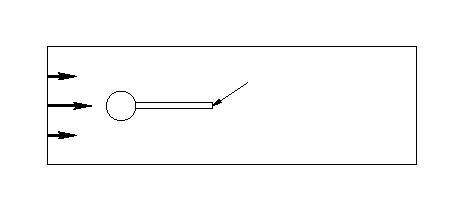
\includegraphics{Pictures/pic_12}%
\end{picture}%
\setlength{\unitlength}{2072sp}%
%
\begingroup\makeatletter\ifx\SetFigFont\undefined%
\gdef\SetFigFont#1#2{%
  \fontsize{#1}{#2pt}%
  \selectfont}%
\fi\endgroup%
\begin{picture}(6330,2785)(3136,-4652)
\put(9001,-4561){\makebox(0,0)[lb]{\smash{{\SetFigFont{8}{9.6}{\color[rgb]{0,0,0}$(2.5,0)$}%
}}}}
\put(9001,-2086){\makebox(0,0)[lb]{\smash{{\SetFigFont{8}{9.6}{\color[rgb]{0,0,0}$(2.5,0.41)$}%
}}}}
\put(3376,-2086){\makebox(0,0)[lb]{\smash{{\SetFigFont{8}{9.6}{\color[rgb]{0,0,0}$(0,0.41)$}%
}}}}
\put(3376,-4561){\makebox(0,0)[lb]{\smash{{\SetFigFont{8}{9.6}{\color[rgb]{0,0,0}$(0,0)$}%
}}}}
\put(6751,-2851){\makebox(0,0)[lb]{\smash{{\SetFigFont{8}{9.6}{\color[rgb]{0,0,0}A=(0.6,0.2)}%
}}}}
\put(7201,-3661){\makebox(0,0)[lb]{\smash{{\SetFigFont{8}{9.6}{\color[rgb]{0,0,0}$\widehat{\Omega}$}%
}}}}
\put(5851,-2086){\makebox(0,0)[lb]{\smash{{\SetFigFont{8}{9.6}{\color[rgb]{0,0,0}$\hat\Gamma_{wall}$}%
}}}}
\put(5851,-4561){\makebox(0,0)[lb]{\smash{{\SetFigFont{8}{9.6}{\color[rgb]{0,0,0}$\hat\Gamma_{wall}$}%
}}}}
\put(3151,-3211){\makebox(0,0)[lb]{\smash{{\SetFigFont{8}{9.6}{\color[rgb]{0,0,0}$\hat\Gamma_{in}$}%
}}}}
\put(9451,-3211){\makebox(0,0)[lb]{\smash{{\SetFigFont{8}{9.6}{\color[rgb]{0,0,0}$\hat\Gamma_{out}$}%
}}}}
\end{picture}%

\caption{Flow around cylinder with elastic beam with 
circle-center $C=(0.2,0.2)$ and radius $r=0.05$.}
\label{configuration_csm_and_fsi_2D}
\end{figure}


The elastic beam has length
$l=0.35m$ and height $h=0.02m$. The right lower end is positioned at 
$(0.6m,0.19m)$, and
the left end is attached to the circle. 
Control points $A(t)$ (with $A(0) = (0.6,0.2)$) are fixed at the 
trailing edge of the structure, measuring $x$- and $y$-deflections of the beam.
Details 
on parameters and evaluation functionals and other results 
can be found in \cite{HrTu06b,BuSc06,Wi11}. 
The time-stepping scheme can be 
very easily chosen in the \texttt{main.cc} function by choosing an appropriate 
time-stepping scheme as explained at the beginning of this manual
and detailed in the previous example.

The quantities of interest are evaluations of 
$x$- and $y$ displacement at the point $A(0) = (0.6,0.2)$
and the drag and lift forces acting on the cylinder and the elastic beam:
\begin{align}
\label{drag_lift_forces}
(F_D , F_L) 
= {\int_{S_f} \hat\sigma_f \cdot \hat n_f \, \mathrm{d}s + 
\int_{\hat\Gamma_i} \hat\sigma_s \cdot \hat n_s \, \mathrm{d}s},
\end{align}
where $S_{f}$ denotes the path over the cylinder in the fluid part and
$\Gamma_i$ the interface between the elastic beam and the 
fluid.

% \begin{table}[h]
%   \small
%   \centering
%     \begin{tabular}{llllcccc}    
%       \hline
%       Configuration & Date         & Refinement & Time dis. & $k$ & $\Delta p$& $F_D$ & $F_L$   \\ \hline\hline
%       BFAC 2D-1     & Mar 10, 2010 & 2 global   & BE        & 1.0    & 0.117412  &       &         \\
%       BFAC 2D-1     & Mar 10, 2010 & 2 global   & FS        & 1.0    & 0.117412  &       &         \\
%       BFAC 2D-1     & Mar 10, 2010 & 2 global   & CN(k)     & 1.0    & 0.117412  &       &         \\ 
%       BFAC 2D-1     & Mar 10, 2010 & 2 global   & CN        & 1.0    & 0.117383  &       &         \\ 
%       BFAC 2D-2     & Mar 10, 2010 & 2 global   & CN(k)     & 1.0    & 2.31541   &       &         \\ 
%       BFAC 2D-2     & Mar 10, 2010 & 3 global   & CN(k)     & 1.0    & 2.32011   &       &         \\   
%       BFAC 2D-2     & Mar 12, 2010 & 3 global   & CN(k)     & 1.0e-2 & 2.50288   &       &         \\   
%     \end{tabular}
%  \end{table}
% 
%\subsubsection{Code validation for FSI with ALE}
%
%The results are summarized below:
%
% \begin{table}[h]
%   \small
%   \centering
%     \begin{tabular}{llllccccc}    
%       \hline
%       Config. & Date & Refinement & Time dis. & $k$ &  $u_x(A) [\times 10^{-5}]$ &$u_y(A) [\times 10^{-4}]$ & $F_D$ & $F_L$  \\ \hline
%       FSI 1   & Mar 12, 2010 & 3 global & BE   & 1.0 & 8.2003  & 2.2732  & &        \\
%       FSI 1   & Apr 08, 2010 & 2 global & BE   & 1.0 & 8.2258  & 2.2813  & &        \\
%       FSI 1   & Apr 08, 2010 & 2 global & CN(k)& 0.5 & 8.2268  & 2.2813  & &        \\
%       FSI 1   & Apr 08, 2010 & 2 global & CN   & 0.5 & 8.2268  & 2.2813  & &        \\
%     \end{tabular}
%  \end{table}
%
%\vspace{0.2cm}
%
\subsubsection{Program description}

The major difference to the first nonstationary program
is the introduction of the 
\begin{verbatim}
void ElementTimeEquationExplicit (...) 
\end{verbatim}
to write all time derivative terms explicitly:
\begin{equation*}
(v^n - v^{n-1}, \phi)_{\Omega}.
\end{equation*}
This behavior is useful since (as shown in the above equations)
other solutions variables have to be considered
around $\partial_t v$ such as $J:=J(u)$. 
The same holds for the corresponding matrix part.

Further, this example shows, how to change the vector behavior, from 
our default option \texttt{fullmem}, where the whole vector is stored in 
the computers main memory. Here, we are only interested in calculating the 
solution once, hence two vectors, one for the current time point and one for the
previous one are sufficient. Hence we choose the option 
\texttt{only\underline{ }recent} so that we don't have to reserve unneccessary memory.
If we need to store the whole trajectory for some reason another option is available 
to circumvent the restrictions due to the size of the main memory, it will be 
described in Example~\ref{PDE_Instat_Black_Scholes}.

\vspace{0.2cm}
